\documentclass[twoside]{book}

% Packages required by doxygen
\usepackage{fixltx2e}
\usepackage{calc}
\usepackage{doxygen}
\usepackage[export]{adjustbox} % also loads graphicx
\usepackage{graphicx}
\usepackage[utf8]{inputenc}
\usepackage{makeidx}
\usepackage{multicol}
\usepackage{multirow}
\PassOptionsToPackage{warn}{textcomp}
\usepackage{textcomp}
\usepackage[nointegrals]{wasysym}
\usepackage[table]{xcolor}

% Font selection
\usepackage[T1]{fontenc}
\usepackage[scaled=.90]{helvet}
\usepackage{courier}
\usepackage{amssymb}
\usepackage{sectsty}
\renewcommand{\familydefault}{\sfdefault}
\allsectionsfont{%
  \fontseries{bc}\selectfont%
  \color{darkgray}%
}
\renewcommand{\DoxyLabelFont}{%
  \fontseries{bc}\selectfont%
  \color{darkgray}%
}
\newcommand{\+}{\discretionary{\mbox{\scriptsize$\hookleftarrow$}}{}{}}

% Page & text layout
\usepackage{geometry}
\geometry{%
  a4paper,%
  top=2.5cm,%
  bottom=2.5cm,%
  left=2.5cm,%
  right=2.5cm%
}
\tolerance=750
\hfuzz=15pt
\hbadness=750
\setlength{\emergencystretch}{15pt}
\setlength{\parindent}{0cm}
\setlength{\parskip}{3ex plus 2ex minus 2ex}
\makeatletter
\renewcommand{\paragraph}{%
  \@startsection{paragraph}{4}{0ex}{-1.0ex}{1.0ex}{%
    \normalfont\normalsize\bfseries\SS@parafont%
  }%
}
\renewcommand{\subparagraph}{%
  \@startsection{subparagraph}{5}{0ex}{-1.0ex}{1.0ex}{%
    \normalfont\normalsize\bfseries\SS@subparafont%
  }%
}
\makeatother

% Headers & footers
\usepackage{fancyhdr}
\pagestyle{fancyplain}
\fancyhead[LE]{\fancyplain{}{\bfseries\thepage}}
\fancyhead[CE]{\fancyplain{}{}}
\fancyhead[RE]{\fancyplain{}{\bfseries\leftmark}}
\fancyhead[LO]{\fancyplain{}{\bfseries\rightmark}}
\fancyhead[CO]{\fancyplain{}{}}
\fancyhead[RO]{\fancyplain{}{\bfseries\thepage}}
\fancyfoot[LE]{\fancyplain{}{}}
\fancyfoot[CE]{\fancyplain{}{}}
\fancyfoot[RE]{\fancyplain{}{\bfseries\scriptsize Generated by Doxygen }}
\fancyfoot[LO]{\fancyplain{}{\bfseries\scriptsize Generated by Doxygen }}
\fancyfoot[CO]{\fancyplain{}{}}
\fancyfoot[RO]{\fancyplain{}{}}
\renewcommand{\footrulewidth}{0.4pt}
\renewcommand{\chaptermark}[1]{%
  \markboth{#1}{}%
}
\renewcommand{\sectionmark}[1]{%
  \markright{\thesection\ #1}%
}

% Indices & bibliography
\usepackage{natbib}
\usepackage[titles]{tocloft}
\setcounter{tocdepth}{3}
\setcounter{secnumdepth}{5}
\makeindex

% Hyperlinks (required, but should be loaded last)
\usepackage{ifpdf}
\ifpdf
  \usepackage[pdftex,pagebackref=true]{hyperref}
\else
  \usepackage[ps2pdf,pagebackref=true]{hyperref}
\fi
\hypersetup{%
  colorlinks=true,%
  linkcolor=blue,%
  citecolor=blue,%
  unicode%
}

% Custom commands
\newcommand{\clearemptydoublepage}{%
  \newpage{\pagestyle{empty}\cleardoublepage}%
}

\usepackage{caption}
\captionsetup{labelsep=space,justification=centering,font={bf},singlelinecheck=off,skip=4pt,position=top}

%===== C O N T E N T S =====

\begin{document}

% Titlepage & ToC
\hypersetup{pageanchor=false,
             bookmarksnumbered=true,
             pdfencoding=unicode
            }
\pagenumbering{alph}
\begin{titlepage}
\vspace*{7cm}
\begin{center}%
{\Large sarah\+G\+UI }\\
\vspace*{1cm}
{\large Generated by Doxygen 1.8.14}\\
\end{center}
\end{titlepage}
\clearemptydoublepage
\pagenumbering{roman}
\tableofcontents
\clearemptydoublepage
\pagenumbering{arabic}
\hypersetup{pageanchor=true}

%--- Begin generated contents ---
\chapter{sarah\+G\+UI}
\label{md__r_e_a_d_m_e}
\Hypertarget{md__r_e_a_d_m_e}
I hate G\+UI, so one day I decided to write some elements once and for all.

Feel free to try to use it, I\textquotesingle{}m building this on linux.

$\sim$$\sim$\# Note\+: I changed one little bit in S\+F\+ML\textquotesingle{}s source before building-\/ set\+Joystick\+Enabled(bool) in sf\+::\+Window. There used to be a bug on windows in which polling the joystick caused the most annoying framerate stutter, but that fixed it. No clue if it still exists, feel free to remove that call in the {\ttfamily \mbox{\hyperlink{class_application}{Application}}} class if it is fixed.$\sim$$\sim$ It was fixed! 
\chapter{Hierarchical Index}
\section{Class Hierarchy}
This inheritance list is sorted roughly, but not completely, alphabetically\+:\begin{DoxyCompactList}
\item \contentsline{section}{Application}{\pageref{class_application}}{}
\item Drawable\begin{DoxyCompactList}
\item \contentsline{section}{Gui\+Component}{\pageref{class_gui_component}}{}
\begin{DoxyCompactList}
\item \contentsline{section}{Gui\+Button}{\pageref{class_gui_button}}{}
\item \contentsline{section}{Gui\+Container}{\pageref{class_gui_container}}{}
\item \contentsline{section}{Gui\+Label}{\pageref{class_gui_label}}{}
\end{DoxyCompactList}
\end{DoxyCompactList}
\item \contentsline{section}{Key\+Manager}{\pageref{class_key_manager}}{}
\item \contentsline{section}{Resource\+Manager}{\pageref{class_resource_manager}}{}
\item Transformable\begin{DoxyCompactList}
\item \contentsline{section}{Gui\+Component}{\pageref{class_gui_component}}{}
\end{DoxyCompactList}
\end{DoxyCompactList}

\chapter{Class Index}
\section{Class List}
Here are the classes, structs, unions and interfaces with brief descriptions\+:\begin{DoxyCompactList}
\item\contentsline{section}{\mbox{\hyperlink{class_application}{Application}} \\*Class to store all application data }{\pageref{class_application}}{}
\item\contentsline{section}{\mbox{\hyperlink{class_gui_button}{Gui\+Button}} \\*Simple G\+UI Button class }{\pageref{class_gui_button}}{}
\item\contentsline{section}{\mbox{\hyperlink{class_gui_component}{Gui\+Component}} \\*Main abstract G\+UI class object. Contains all base methods to manage children \& the parent object, for a tree-\/like G\+UI structure }{\pageref{class_gui_component}}{}
\item\contentsline{section}{\mbox{\hyperlink{class_gui_container}{Gui\+Container}} \\*Base container class, provides an organized border to house more complex G\+UI elements }{\pageref{class_gui_container}}{}
\item\contentsline{section}{\mbox{\hyperlink{class_gui_label}{Gui\+Label}} \\*G\+UI component for displaying \& updating simple text }{\pageref{class_gui_label}}{}
\item\contentsline{section}{\mbox{\hyperlink{class_key_manager}{Key\+Manager}} \\*Simple mostly static \mbox{\hyperlink{class_key_manager}{Key\+Manager}} class for retrieving the state of the keyboard \& mouse globally }{\pageref{class_key_manager}}{}
\item\contentsline{section}{\mbox{\hyperlink{class_resource_manager}{Resource\+Manager}} \\*Class to manage resources to avoid loading the same file twice }{\pageref{class_resource_manager}}{}
\end{DoxyCompactList}

\chapter{Class Documentation}
\hypertarget{class_application}{}\section{Application Class Reference}
\label{class_application}\index{Application@{Application}}


Class to store all application data.  




{\ttfamily \#include $<$Application.\+h$>$}

\subsection*{Public Member Functions}
\begin{DoxyCompactItemize}
\item 
\mbox{\Hypertarget{class_application_afa8cc05ce6b6092be5ecdfdae44e05f8}\label{class_application_afa8cc05ce6b6092be5ecdfdae44e05f8}} 
\mbox{\hyperlink{class_application_afa8cc05ce6b6092be5ecdfdae44e05f8}{Application}} ()
\begin{DoxyCompactList}\small\item\em Default Constructor. \end{DoxyCompactList}\item 
int \mbox{\hyperlink{class_application_a8cf8941c8db90117d3735bce5ae1fdf4}{run}} ()
\begin{DoxyCompactList}\small\item\em The main application loop. \end{DoxyCompactList}\end{DoxyCompactItemize}


\subsection{Detailed Description}
Class to store all application data. 

\subsection{Member Function Documentation}
\mbox{\Hypertarget{class_application_a8cf8941c8db90117d3735bce5ae1fdf4}\label{class_application_a8cf8941c8db90117d3735bce5ae1fdf4}} 
\index{Application@{Application}!run@{run}}
\index{run@{run}!Application@{Application}}
\subsubsection{\texorpdfstring{run()}{run()}}
{\footnotesize\ttfamily int Application\+::run (\begin{DoxyParamCaption}{ }\end{DoxyParamCaption})}



The main application loop. 

\begin{DoxyReturn}{Returns}
int The program\textquotesingle{}s exit code. 
\end{DoxyReturn}


The documentation for this class was generated from the following files\+:\begin{DoxyCompactItemize}
\item 
header/Application.\+h\item 
src/Application.\+cpp\end{DoxyCompactItemize}

\hypertarget{class_gui_button}{}\section{Gui\+Button Class Reference}
\label{class_gui_button}\index{Gui\+Button@{Gui\+Button}}
Inheritance diagram for Gui\+Button\+:\begin{figure}[H]
\begin{center}
\leavevmode
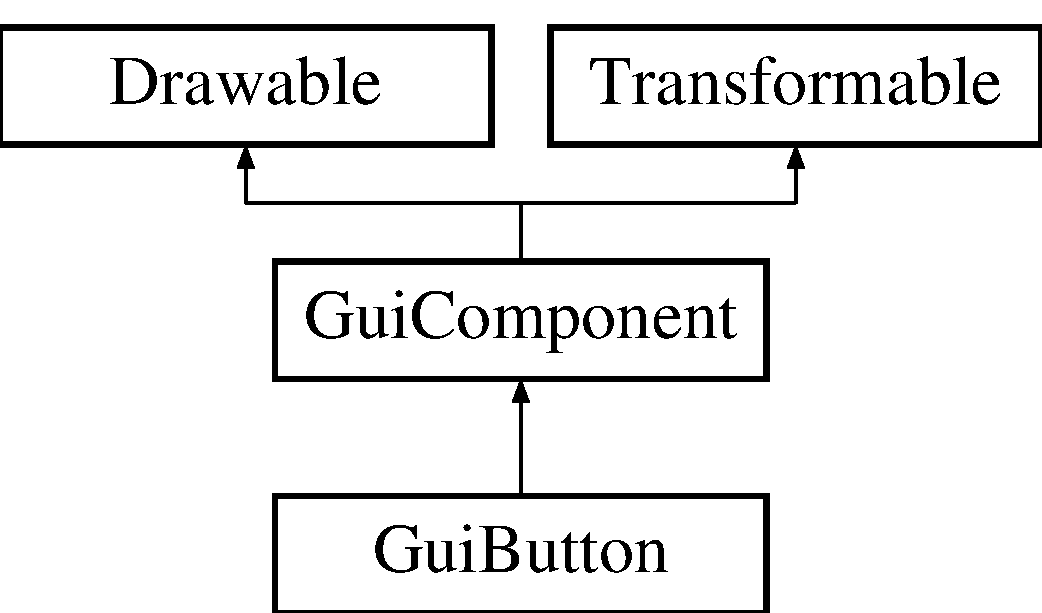
\includegraphics[height=3.000000cm]{class_gui_button}
\end{center}
\end{figure}
\subsection*{Additional Inherited Members}


The documentation for this class was generated from the following file\+:\begin{DoxyCompactItemize}
\item 
header/Gui\+Button.\+h\end{DoxyCompactItemize}

\hypertarget{class_gui_component}{}\section{Gui\+Component Class Reference}
\label{class_gui_component}\index{Gui\+Component@{Gui\+Component}}


Main abstract G\+UI class object. Contains all base methods to manage children \& the parent object, for a tree-\/like G\+UI structure.  




{\ttfamily \#include $<$Gui\+Component.\+h$>$}

Inheritance diagram for Gui\+Component\+:\begin{figure}[H]
\begin{center}
\leavevmode
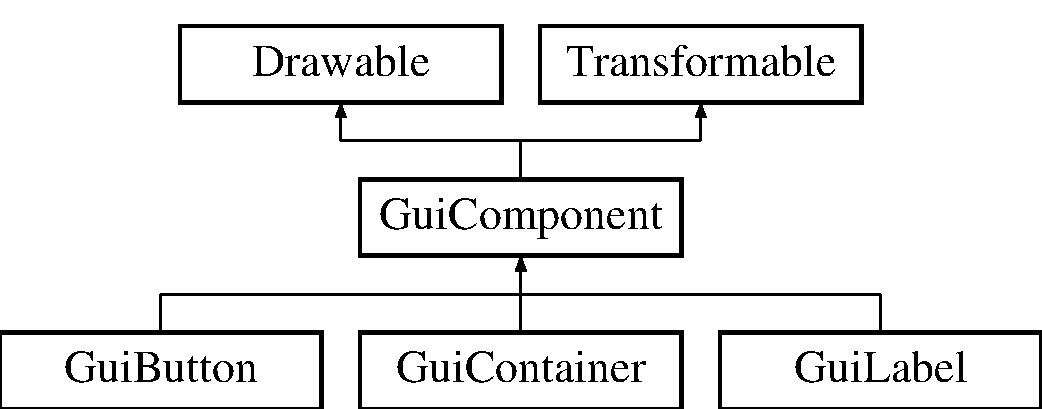
\includegraphics[height=3.000000cm]{class_gui_component}
\end{center}
\end{figure}
\subsection*{Public Member Functions}
\begin{DoxyCompactItemize}
\item 
\mbox{\Hypertarget{class_gui_component_a39e1734c781ba4ac8c87da58e0a10ebd}\label{class_gui_component_a39e1734c781ba4ac8c87da58e0a10ebd}} 
\mbox{\hyperlink{class_gui_component_a39e1734c781ba4ac8c87da58e0a10ebd}{Gui\+Component}} ()
\begin{DoxyCompactList}\small\item\em Default Constructor. \end{DoxyCompactList}\item 
\mbox{\Hypertarget{class_gui_component_ad94998891efad935b4422cf1da69e4af}\label{class_gui_component_ad94998891efad935b4422cf1da69e4af}} 
virtual \mbox{\hyperlink{class_gui_component_ad94998891efad935b4422cf1da69e4af}{$\sim$\+Gui\+Component}} ()
\begin{DoxyCompactList}\small\item\em Virtual Destructor. \end{DoxyCompactList}\item 
\mbox{\Hypertarget{class_gui_component_ac58e20a01f67cf605b069ef853dfab66}\label{class_gui_component_ac58e20a01f67cf605b069ef853dfab66}} 
void \mbox{\hyperlink{class_gui_component_ac58e20a01f67cf605b069ef853dfab66}{update\+Recursive}} ()
\begin{DoxyCompactList}\small\item\em Calls this-\/$>$\mbox{\hyperlink{class_gui_component_adacaca1d0604e6b93cb22962e60cc285}{update()}}, as well as all childrens\textquotesingle{} \mbox{\hyperlink{class_gui_component_ac58e20a01f67cf605b069ef853dfab66}{update\+Recursive()}}, updating all child objects with one parent call. \end{DoxyCompactList}\item 
virtual void \mbox{\hyperlink{class_gui_component_adacaca1d0604e6b93cb22962e60cc285}{update}} ()
\begin{DoxyCompactList}\small\item\em Update this \& only this object, no children. \end{DoxyCompactList}\item 
\mbox{\Hypertarget{class_gui_component_a7c42118c5d2ba58ca02a1ea5ff81fe78}\label{class_gui_component_a7c42118c5d2ba58ca02a1ea5ff81fe78}} 
virtual void \mbox{\hyperlink{class_gui_component_a7c42118c5d2ba58ca02a1ea5ff81fe78}{rm\+\_\+init}} (\mbox{\hyperlink{class_resource_manager}{Resource\+Manager}} \&)=0
\begin{DoxyCompactList}\small\item\em Called by \mbox{\hyperlink{class_resource_manager_ad543c034d0cef8fd2f3e8f32b49ebb3f}{Resource\+Manager.\+init\+Object()}}, inherit \& override to initialize textures \& resources. \end{DoxyCompactList}\item 
void \mbox{\hyperlink{class_gui_component_a526481fb2424c1ea771e78be27a091f9}{set\+Parent}} (\mbox{\hyperlink{class_gui_component}{Gui\+Component}} $\ast$parent)
\begin{DoxyCompactList}\small\item\em Set this object\textquotesingle{}s parent. Usually called from the parent\textquotesingle{}s \mbox{\hyperlink{class_gui_component_a5bccaccef3d0eab8af3be84cab1300de}{add\+Child()}} method. \end{DoxyCompactList}\item 
\mbox{\hyperlink{class_gui_component}{Gui\+Component}} $\ast$ \mbox{\hyperlink{class_gui_component_aba1969f731ef56396a1e69e50ff1f8fb}{get\+Parent}} ()
\begin{DoxyCompactList}\small\item\em Get this object\textquotesingle{}s parent. \end{DoxyCompactList}\item 
sf\+::\+Transform \mbox{\hyperlink{class_gui_component_a9402e70432502a9b8187365a95839a05}{get\+Full\+Transform}} ()
\begin{DoxyCompactList}\small\item\em Get the combined transformation of this object\textquotesingle{}s parent \& all parents above. \end{DoxyCompactList}\item 
virtual void \mbox{\hyperlink{class_gui_component_a5bccaccef3d0eab8af3be84cab1300de}{add\+Child}} (\mbox{\hyperlink{class_gui_component}{Gui\+Component}} $\ast$new\+Child)
\begin{DoxyCompactList}\small\item\em Pushes the object into the vector of children. Also calls \mbox{\hyperlink{class_gui_component_a526481fb2424c1ea771e78be27a091f9}{set\+Parent()}} on the child object. \end{DoxyCompactList}\item 
virtual void \mbox{\hyperlink{class_gui_component_ac979fb459db6feda90bc7c11a6a60623}{remove\+Child}} (std\+::string name)
\begin{DoxyCompactList}\small\item\em Removes a child from the list of children by name. \end{DoxyCompactList}\item 
\mbox{\Hypertarget{class_gui_component_ac8fea01fa84d85bc1e511211f74cfd53}\label{class_gui_component_ac8fea01fa84d85bc1e511211f74cfd53}} 
virtual void \mbox{\hyperlink{class_gui_component_ac8fea01fa84d85bc1e511211f74cfd53}{remove\+Children}} ()
\begin{DoxyCompactList}\small\item\em Completely removes all children. \end{DoxyCompactList}\item 
virtual \mbox{\hyperlink{class_gui_component}{Gui\+Component}} $\ast$ \mbox{\hyperlink{class_gui_component_a2167444f909f08b7be3805309d7ad831}{search\+Child}} (std\+::string name)
\begin{DoxyCompactList}\small\item\em Searches \& retrieves a child by name, locally. Does not search children of children. \end{DoxyCompactList}\item 
virtual \mbox{\hyperlink{class_gui_component}{Gui\+Component}} $\ast$ \mbox{\hyperlink{class_gui_component_a7f1e0e731d458135182850a53de06f95}{search\+Child\+Recursive}} (std\+::string name)
\begin{DoxyCompactList}\small\item\em Searches for children recursively through the whole G\+UI tree. \end{DoxyCompactList}\item 
std\+::string \mbox{\hyperlink{class_gui_component_a521f21d8ae5369fe255a1209fcd3bd0f}{get\+Name}} ()
\begin{DoxyCompactList}\small\item\em Retrieves the name of this object. \end{DoxyCompactList}\item 
void \mbox{\hyperlink{class_gui_component_ae673013e55aa98c6ee267fad3e282766}{set\+Name}} (std\+::string new\+Name)
\begin{DoxyCompactList}\small\item\em Sets the name. \end{DoxyCompactList}\end{DoxyCompactItemize}
\subsection*{Protected Attributes}
\begin{DoxyCompactItemize}
\item 
\mbox{\Hypertarget{class_gui_component_ad25e337a93c4b506634e5766cc46ef4a}\label{class_gui_component_ad25e337a93c4b506634e5766cc46ef4a}} 
\mbox{\hyperlink{class_gui_component}{Gui\+Component}} $\ast$ \mbox{\hyperlink{class_gui_component_ad25e337a93c4b506634e5766cc46ef4a}{m\+Parent}}
\begin{DoxyCompactList}\small\item\em This object\textquotesingle{}s parent. \end{DoxyCompactList}\item 
\mbox{\Hypertarget{class_gui_component_a040e49b543fd6a36b1e0133a5e8dbd3d}\label{class_gui_component_a040e49b543fd6a36b1e0133a5e8dbd3d}} 
std\+::vector$<$ \mbox{\hyperlink{class_gui_component}{Gui\+Component}} $\ast$ $>$ \mbox{\hyperlink{class_gui_component_a040e49b543fd6a36b1e0133a5e8dbd3d}{m\+Children}}
\begin{DoxyCompactList}\small\item\em The vector of children. \end{DoxyCompactList}\end{DoxyCompactItemize}


\subsection{Detailed Description}
Main abstract G\+UI class object. Contains all base methods to manage children \& the parent object, for a tree-\/like G\+UI structure. 

\subsection{Member Function Documentation}
\mbox{\Hypertarget{class_gui_component_a5bccaccef3d0eab8af3be84cab1300de}\label{class_gui_component_a5bccaccef3d0eab8af3be84cab1300de}} 
\index{Gui\+Component@{Gui\+Component}!add\+Child@{add\+Child}}
\index{add\+Child@{add\+Child}!Gui\+Component@{Gui\+Component}}
\subsubsection{\texorpdfstring{add\+Child()}{addChild()}}
{\footnotesize\ttfamily void Gui\+Component\+::add\+Child (\begin{DoxyParamCaption}\item[{\mbox{\hyperlink{class_gui_component}{Gui\+Component}} $\ast$}]{new\+Child }\end{DoxyParamCaption})\hspace{0.3cm}{\ttfamily [virtual]}}



Pushes the object into the vector of children. Also calls \mbox{\hyperlink{class_gui_component_a526481fb2424c1ea771e78be27a091f9}{set\+Parent()}} on the child object. 


\begin{DoxyParams}{Parameters}
{\em new\+Child} & The child to associate. \\
\hline
\end{DoxyParams}
\mbox{\Hypertarget{class_gui_component_a9402e70432502a9b8187365a95839a05}\label{class_gui_component_a9402e70432502a9b8187365a95839a05}} 
\index{Gui\+Component@{Gui\+Component}!get\+Full\+Transform@{get\+Full\+Transform}}
\index{get\+Full\+Transform@{get\+Full\+Transform}!Gui\+Component@{Gui\+Component}}
\subsubsection{\texorpdfstring{get\+Full\+Transform()}{getFullTransform()}}
{\footnotesize\ttfamily sf\+::\+Transform Gui\+Component\+::get\+Full\+Transform (\begin{DoxyParamCaption}{ }\end{DoxyParamCaption})}



Get the combined transformation of this object\textquotesingle{}s parent \& all parents above. 

\begin{DoxyReturn}{Returns}
sf\+::\+Transform The sum transform of all elements up to the top of the tree. 
\end{DoxyReturn}
\mbox{\Hypertarget{class_gui_component_a521f21d8ae5369fe255a1209fcd3bd0f}\label{class_gui_component_a521f21d8ae5369fe255a1209fcd3bd0f}} 
\index{Gui\+Component@{Gui\+Component}!get\+Name@{get\+Name}}
\index{get\+Name@{get\+Name}!Gui\+Component@{Gui\+Component}}
\subsubsection{\texorpdfstring{get\+Name()}{getName()}}
{\footnotesize\ttfamily std\+::string Gui\+Component\+::get\+Name (\begin{DoxyParamCaption}{ }\end{DoxyParamCaption})}



Retrieves the name of this object. 

\begin{DoxyReturn}{Returns}
std\+::string The name of this object. 
\end{DoxyReturn}
\mbox{\Hypertarget{class_gui_component_aba1969f731ef56396a1e69e50ff1f8fb}\label{class_gui_component_aba1969f731ef56396a1e69e50ff1f8fb}} 
\index{Gui\+Component@{Gui\+Component}!get\+Parent@{get\+Parent}}
\index{get\+Parent@{get\+Parent}!Gui\+Component@{Gui\+Component}}
\subsubsection{\texorpdfstring{get\+Parent()}{getParent()}}
{\footnotesize\ttfamily \mbox{\hyperlink{class_gui_component}{Gui\+Component}} $\ast$ Gui\+Component\+::get\+Parent (\begin{DoxyParamCaption}{ }\end{DoxyParamCaption})}



Get this object\textquotesingle{}s parent. 

\begin{DoxyReturn}{Returns}
Gui\+Component$\ast$ A pointer to the parent object. 
\end{DoxyReturn}
\mbox{\Hypertarget{class_gui_component_ac979fb459db6feda90bc7c11a6a60623}\label{class_gui_component_ac979fb459db6feda90bc7c11a6a60623}} 
\index{Gui\+Component@{Gui\+Component}!remove\+Child@{remove\+Child}}
\index{remove\+Child@{remove\+Child}!Gui\+Component@{Gui\+Component}}
\subsubsection{\texorpdfstring{remove\+Child()}{removeChild()}}
{\footnotesize\ttfamily void Gui\+Component\+::remove\+Child (\begin{DoxyParamCaption}\item[{std\+::string}]{name }\end{DoxyParamCaption})\hspace{0.3cm}{\ttfamily [virtual]}}



Removes a child from the list of children by name. 


\begin{DoxyParams}{Parameters}
{\em name} & The child\textquotesingle{}s name to remove. \\
\hline
\end{DoxyParams}
\mbox{\Hypertarget{class_gui_component_a2167444f909f08b7be3805309d7ad831}\label{class_gui_component_a2167444f909f08b7be3805309d7ad831}} 
\index{Gui\+Component@{Gui\+Component}!search\+Child@{search\+Child}}
\index{search\+Child@{search\+Child}!Gui\+Component@{Gui\+Component}}
\subsubsection{\texorpdfstring{search\+Child()}{searchChild()}}
{\footnotesize\ttfamily \mbox{\hyperlink{class_gui_component}{Gui\+Component}} $\ast$ Gui\+Component\+::search\+Child (\begin{DoxyParamCaption}\item[{std\+::string}]{name }\end{DoxyParamCaption})\hspace{0.3cm}{\ttfamily [virtual]}}



Searches \& retrieves a child by name, locally. Does not search children of children. 


\begin{DoxyParams}{Parameters}
{\em name} & The name of the child to search for. \\
\hline
\end{DoxyParams}
\begin{DoxyReturn}{Returns}
Gui\+Component$\ast$ Either the child requested, or nullptr if it doesn\textquotesingle{}t exist. 
\end{DoxyReturn}
\mbox{\Hypertarget{class_gui_component_a7f1e0e731d458135182850a53de06f95}\label{class_gui_component_a7f1e0e731d458135182850a53de06f95}} 
\index{Gui\+Component@{Gui\+Component}!search\+Child\+Recursive@{search\+Child\+Recursive}}
\index{search\+Child\+Recursive@{search\+Child\+Recursive}!Gui\+Component@{Gui\+Component}}
\subsubsection{\texorpdfstring{search\+Child\+Recursive()}{searchChildRecursive()}}
{\footnotesize\ttfamily \mbox{\hyperlink{class_gui_component}{Gui\+Component}} $\ast$ Gui\+Component\+::search\+Child\+Recursive (\begin{DoxyParamCaption}\item[{std\+::string}]{name }\end{DoxyParamCaption})\hspace{0.3cm}{\ttfamily [virtual]}}



Searches for children recursively through the whole G\+UI tree. 


\begin{DoxyParams}{Parameters}
{\em name} & The name of the child to retrieve. \\
\hline
\end{DoxyParams}
\begin{DoxyReturn}{Returns}
Gui\+Component$\ast$ The child to retrieve, or nullptr if the name is not registered. 
\end{DoxyReturn}
\mbox{\Hypertarget{class_gui_component_ae673013e55aa98c6ee267fad3e282766}\label{class_gui_component_ae673013e55aa98c6ee267fad3e282766}} 
\index{Gui\+Component@{Gui\+Component}!set\+Name@{set\+Name}}
\index{set\+Name@{set\+Name}!Gui\+Component@{Gui\+Component}}
\subsubsection{\texorpdfstring{set\+Name()}{setName()}}
{\footnotesize\ttfamily void Gui\+Component\+::set\+Name (\begin{DoxyParamCaption}\item[{std\+::string}]{new\+Name }\end{DoxyParamCaption})}



Sets the name. 


\begin{DoxyParams}{Parameters}
{\em new\+Name} & The new name. \\
\hline
\end{DoxyParams}
\mbox{\Hypertarget{class_gui_component_a526481fb2424c1ea771e78be27a091f9}\label{class_gui_component_a526481fb2424c1ea771e78be27a091f9}} 
\index{Gui\+Component@{Gui\+Component}!set\+Parent@{set\+Parent}}
\index{set\+Parent@{set\+Parent}!Gui\+Component@{Gui\+Component}}
\subsubsection{\texorpdfstring{set\+Parent()}{setParent()}}
{\footnotesize\ttfamily void Gui\+Component\+::set\+Parent (\begin{DoxyParamCaption}\item[{\mbox{\hyperlink{class_gui_component}{Gui\+Component}} $\ast$}]{parent }\end{DoxyParamCaption})}



Set this object\textquotesingle{}s parent. Usually called from the parent\textquotesingle{}s \mbox{\hyperlink{class_gui_component_a5bccaccef3d0eab8af3be84cab1300de}{add\+Child()}} method. 


\begin{DoxyParams}{Parameters}
{\em parent} & The parent object. \\
\hline
\end{DoxyParams}
\mbox{\Hypertarget{class_gui_component_adacaca1d0604e6b93cb22962e60cc285}\label{class_gui_component_adacaca1d0604e6b93cb22962e60cc285}} 
\index{Gui\+Component@{Gui\+Component}!update@{update}}
\index{update@{update}!Gui\+Component@{Gui\+Component}}
\subsubsection{\texorpdfstring{update()}{update()}}
{\footnotesize\ttfamily void Gui\+Component\+::update (\begin{DoxyParamCaption}{ }\end{DoxyParamCaption})\hspace{0.3cm}{\ttfamily [virtual]}}



Update this \& only this object, no children. 

\begin{DoxyRemark}{Remarks}
Usually only called by \mbox{\hyperlink{class_gui_component_ac58e20a01f67cf605b069ef853dfab66}{update\+Recursive()}}, but no harm should be causable by only calling this. Try not to mix calls. 
\end{DoxyRemark}


Reimplemented in \mbox{\hyperlink{class_gui_button_afd7f69faf6201309727bce6ff9d04f56}{Gui\+Button}}.



The documentation for this class was generated from the following files\+:\begin{DoxyCompactItemize}
\item 
header/Gui\+Component.\+h\item 
src/Gui\+Component.\+cpp\end{DoxyCompactItemize}

\hypertarget{class_gui_container}{}\section{Gui\+Container Class Reference}
\label{class_gui_container}\index{Gui\+Container@{Gui\+Container}}


Base container class, provides an organized border to house more complex G\+UI elements.  




{\ttfamily \#include $<$Gui\+Container.\+h$>$}

Inheritance diagram for Gui\+Container\+:\begin{figure}[H]
\begin{center}
\leavevmode
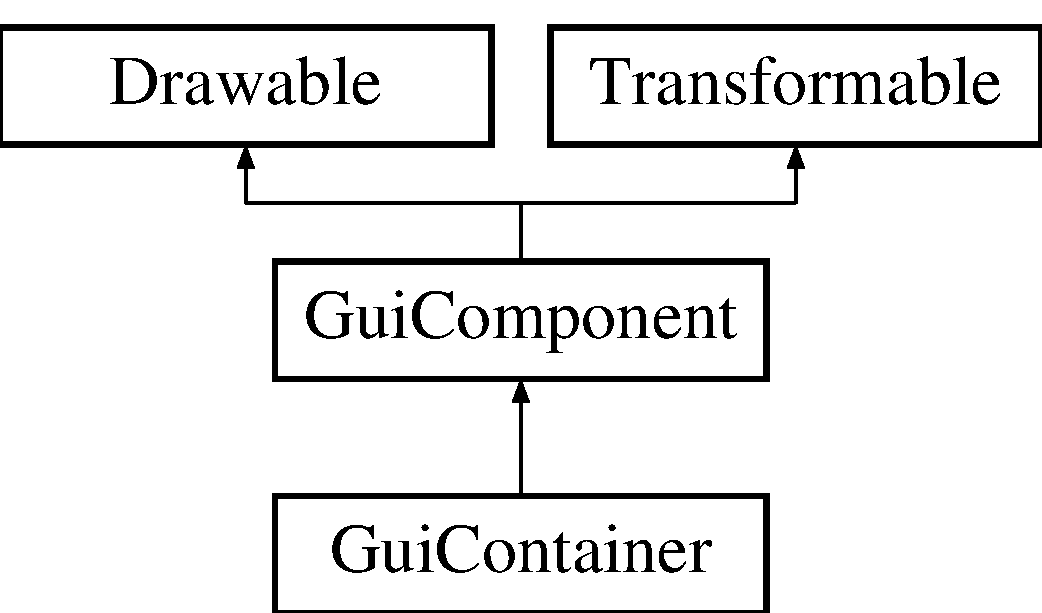
\includegraphics[height=3.000000cm]{class_gui_container}
\end{center}
\end{figure}
\subsection*{Public Member Functions}
\begin{DoxyCompactItemize}
\item 
\mbox{\Hypertarget{class_gui_container_aa76c191132371ff7186ca5ef344da9bd}\label{class_gui_container_aa76c191132371ff7186ca5ef344da9bd}} 
\mbox{\hyperlink{class_gui_container_aa76c191132371ff7186ca5ef344da9bd}{Gui\+Container}} ()
\begin{DoxyCompactList}\small\item\em Default Constructor. \end{DoxyCompactList}\item 
void \mbox{\hyperlink{class_gui_container_af800879fd21fae9d7fef5257fb1fcd5e}{rm\+\_\+init}} (\mbox{\hyperlink{class_resource_manager}{Resource\+Manager}} \&r)
\begin{DoxyCompactList}\small\item\em The resource initialization function. \end{DoxyCompactList}\end{DoxyCompactItemize}
\subsection*{Additional Inherited Members}


\subsection{Detailed Description}
Base container class, provides an organized border to house more complex G\+UI elements. 

\subsection{Member Function Documentation}
\mbox{\Hypertarget{class_gui_container_af800879fd21fae9d7fef5257fb1fcd5e}\label{class_gui_container_af800879fd21fae9d7fef5257fb1fcd5e}} 
\index{Gui\+Container@{Gui\+Container}!rm\+\_\+init@{rm\+\_\+init}}
\index{rm\+\_\+init@{rm\+\_\+init}!Gui\+Container@{Gui\+Container}}
\subsubsection{\texorpdfstring{rm\+\_\+init()}{rm\_init()}}
{\footnotesize\ttfamily void Gui\+Container\+::rm\+\_\+init (\begin{DoxyParamCaption}\item[{\mbox{\hyperlink{class_resource_manager}{Resource\+Manager}} \&}]{r }\end{DoxyParamCaption})\hspace{0.3cm}{\ttfamily [virtual]}}



The resource initialization function. 


\begin{DoxyParams}{Parameters}
{\em r} & Reference to the global resource manager. \\
\hline
\end{DoxyParams}


Implements \mbox{\hyperlink{class_gui_component_a7c42118c5d2ba58ca02a1ea5ff81fe78}{Gui\+Component}}.



The documentation for this class was generated from the following files\+:\begin{DoxyCompactItemize}
\item 
header/Gui\+Container.\+h\item 
src/Gui\+Container.\+cpp\end{DoxyCompactItemize}

\hypertarget{class_gui_label}{}\section{Gui\+Label Class Reference}
\label{class_gui_label}\index{Gui\+Label@{Gui\+Label}}


G\+UI component for displaying \& updating simple text.  




{\ttfamily \#include $<$Gui\+Label.\+h$>$}

Inheritance diagram for Gui\+Label\+:\begin{figure}[H]
\begin{center}
\leavevmode
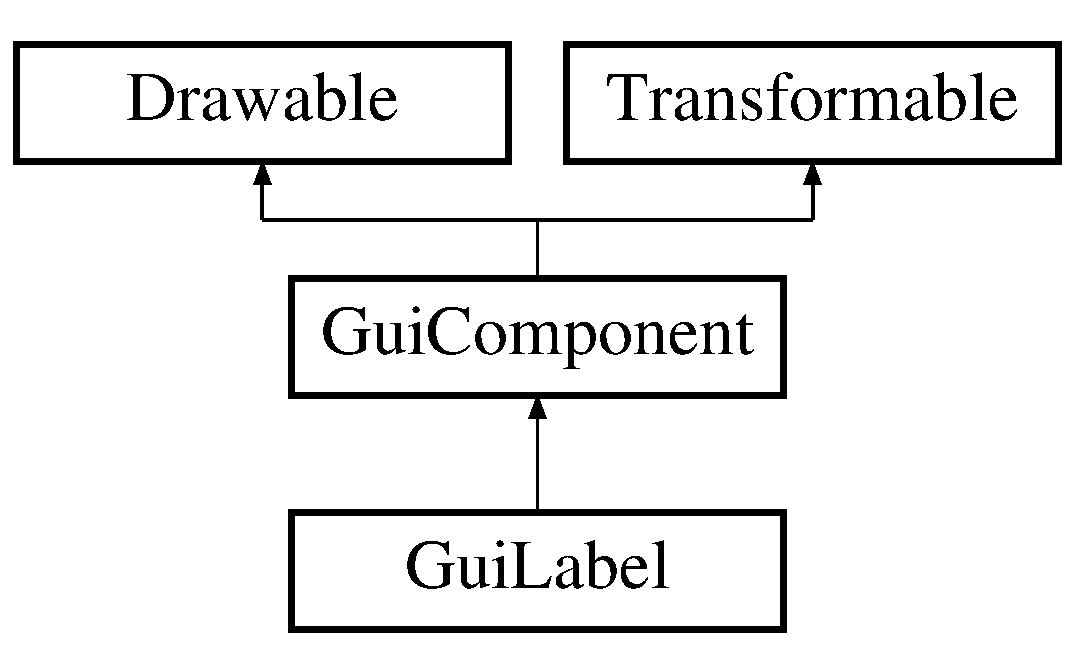
\includegraphics[height=3.000000cm]{class_gui_label}
\end{center}
\end{figure}
\subsection*{Public Types}
\begin{DoxyCompactItemize}
\item 
\mbox{\Hypertarget{class_gui_label_a408cd142a14adb06d632ed44e674ddf2}\label{class_gui_label_a408cd142a14adb06d632ed44e674ddf2}} 
enum \mbox{\hyperlink{class_gui_label_a408cd142a14adb06d632ed44e674ddf2}{Align}} \{ \newline
{\bfseries T\+O\+P\+\_\+\+L\+E\+FT}, 
{\bfseries T\+O\+P\+\_\+\+M\+I\+D\+D\+LE}, 
{\bfseries T\+O\+P\+\_\+\+R\+I\+G\+HT}, 
{\bfseries M\+I\+D\+D\+L\+E\+\_\+\+L\+E\+FT}, 
\newline
{\bfseries M\+I\+D\+D\+L\+E\+\_\+\+M\+I\+D\+D\+LE}, 
{\bfseries M\+I\+D\+D\+L\+E\+\_\+\+R\+I\+G\+HT}, 
{\bfseries B\+O\+T\+T\+O\+M\+\_\+\+L\+E\+FT}, 
{\bfseries B\+O\+T\+T\+O\+M\+\_\+\+M\+I\+D\+D\+LE}, 
\newline
{\bfseries B\+O\+T\+T\+O\+M\+\_\+\+R\+I\+G\+HT}
 \}
\begin{DoxyCompactList}\small\item\em Alignment enum, for aligning text. \end{DoxyCompactList}\end{DoxyCompactItemize}
\subsection*{Public Member Functions}
\begin{DoxyCompactItemize}
\item 
\mbox{\Hypertarget{class_gui_label_aa996ad603e5692673485780ee6b6bf27}\label{class_gui_label_aa996ad603e5692673485780ee6b6bf27}} 
\mbox{\hyperlink{class_gui_label_aa996ad603e5692673485780ee6b6bf27}{Gui\+Label}} ()
\begin{DoxyCompactList}\small\item\em Default Constructor. \end{DoxyCompactList}\item 
void \mbox{\hyperlink{class_gui_label_afa1cce21b5bfaba22076619ec635de84}{rm\+\_\+init}} (\mbox{\hyperlink{class_resource_manager}{Resource\+Manager}} \&r)
\begin{DoxyCompactList}\small\item\em Resource initialization for init\+Object() \end{DoxyCompactList}\item 
void \mbox{\hyperlink{class_gui_label_a40dcdb9bc406ab8ecee7e1e6df69c989}{set\+String}} (std\+::string new\+String)
\begin{DoxyCompactList}\small\item\em Set the text displayed. \end{DoxyCompactList}\item 
std\+::string \mbox{\hyperlink{class_gui_label_ade16f5556300d8c353f7c45684bd75eb}{get\+String}} ()
\begin{DoxyCompactList}\small\item\em Retrieve the currently displayed text. \end{DoxyCompactList}\item 
void \mbox{\hyperlink{class_gui_label_ab0eaf82245f1271dd8e261fd306647b1}{set\+Character\+Size}} (unsigned short n)
\begin{DoxyCompactList}\small\item\em Set the font\textquotesingle{}s character size. \end{DoxyCompactList}\item 
void \mbox{\hyperlink{class_gui_label_ae9ba2f0ceb51fbe073ba8fc297288aff}{update\+Alignment}} (\mbox{\hyperlink{class_gui_label_a408cd142a14adb06d632ed44e674ddf2}{Align}} new\+Align)
\begin{DoxyCompactList}\small\item\em Update the alignment of the text. \end{DoxyCompactList}\end{DoxyCompactItemize}
\subsection*{Additional Inherited Members}


\subsection{Detailed Description}
G\+UI component for displaying \& updating simple text. 

\subsection{Member Function Documentation}
\mbox{\Hypertarget{class_gui_label_ade16f5556300d8c353f7c45684bd75eb}\label{class_gui_label_ade16f5556300d8c353f7c45684bd75eb}} 
\index{Gui\+Label@{Gui\+Label}!get\+String@{get\+String}}
\index{get\+String@{get\+String}!Gui\+Label@{Gui\+Label}}
\subsubsection{\texorpdfstring{get\+String()}{getString()}}
{\footnotesize\ttfamily std\+::string Gui\+Label\+::get\+String (\begin{DoxyParamCaption}{ }\end{DoxyParamCaption})}



Retrieve the currently displayed text. 

\begin{DoxyReturn}{Returns}
std\+::string The current text. 
\end{DoxyReturn}
\mbox{\Hypertarget{class_gui_label_afa1cce21b5bfaba22076619ec635de84}\label{class_gui_label_afa1cce21b5bfaba22076619ec635de84}} 
\index{Gui\+Label@{Gui\+Label}!rm\+\_\+init@{rm\+\_\+init}}
\index{rm\+\_\+init@{rm\+\_\+init}!Gui\+Label@{Gui\+Label}}
\subsubsection{\texorpdfstring{rm\+\_\+init()}{rm\_init()}}
{\footnotesize\ttfamily void Gui\+Label\+::rm\+\_\+init (\begin{DoxyParamCaption}\item[{\mbox{\hyperlink{class_resource_manager}{Resource\+Manager}} \&}]{r }\end{DoxyParamCaption})\hspace{0.3cm}{\ttfamily [virtual]}}



Resource initialization for init\+Object() 


\begin{DoxyParams}{Parameters}
{\em r} & The global resource manager. \\
\hline
\end{DoxyParams}


Implements \mbox{\hyperlink{class_gui_component_a7c42118c5d2ba58ca02a1ea5ff81fe78}{Gui\+Component}}.

\mbox{\Hypertarget{class_gui_label_ab0eaf82245f1271dd8e261fd306647b1}\label{class_gui_label_ab0eaf82245f1271dd8e261fd306647b1}} 
\index{Gui\+Label@{Gui\+Label}!set\+Character\+Size@{set\+Character\+Size}}
\index{set\+Character\+Size@{set\+Character\+Size}!Gui\+Label@{Gui\+Label}}
\subsubsection{\texorpdfstring{set\+Character\+Size()}{setCharacterSize()}}
{\footnotesize\ttfamily void Gui\+Label\+::set\+Character\+Size (\begin{DoxyParamCaption}\item[{unsigned short}]{n }\end{DoxyParamCaption})}



Set the font\textquotesingle{}s character size. 


\begin{DoxyParams}{Parameters}
{\em n} & The new font size. \\
\hline
\end{DoxyParams}
\mbox{\Hypertarget{class_gui_label_a40dcdb9bc406ab8ecee7e1e6df69c989}\label{class_gui_label_a40dcdb9bc406ab8ecee7e1e6df69c989}} 
\index{Gui\+Label@{Gui\+Label}!set\+String@{set\+String}}
\index{set\+String@{set\+String}!Gui\+Label@{Gui\+Label}}
\subsubsection{\texorpdfstring{set\+String()}{setString()}}
{\footnotesize\ttfamily void Gui\+Label\+::set\+String (\begin{DoxyParamCaption}\item[{std\+::string}]{new\+String }\end{DoxyParamCaption})}



Set the text displayed. 


\begin{DoxyParams}{Parameters}
{\em new\+String} & The new text to show. \\
\hline
\end{DoxyParams}
\mbox{\Hypertarget{class_gui_label_ae9ba2f0ceb51fbe073ba8fc297288aff}\label{class_gui_label_ae9ba2f0ceb51fbe073ba8fc297288aff}} 
\index{Gui\+Label@{Gui\+Label}!update\+Alignment@{update\+Alignment}}
\index{update\+Alignment@{update\+Alignment}!Gui\+Label@{Gui\+Label}}
\subsubsection{\texorpdfstring{update\+Alignment()}{updateAlignment()}}
{\footnotesize\ttfamily void Gui\+Label\+::update\+Alignment (\begin{DoxyParamCaption}\item[{\mbox{\hyperlink{class_gui_label_a408cd142a14adb06d632ed44e674ddf2}{Align}}}]{new\+Align }\end{DoxyParamCaption})}



Update the alignment of the text. 


\begin{DoxyParams}{Parameters}
{\em new\+Align} & The new alignment to configure the text to. \\
\hline
\end{DoxyParams}


The documentation for this class was generated from the following files\+:\begin{DoxyCompactItemize}
\item 
header/Gui\+Label.\+h\item 
src/Gui\+Label.\+cpp\end{DoxyCompactItemize}

\hypertarget{class_key_manager}{}\section{Key\+Manager Class Reference}
\label{class_key_manager}\index{Key\+Manager@{Key\+Manager}}


Simple mostly static \mbox{\hyperlink{class_key_manager}{Key\+Manager}} class for retrieving the state of the keyboard \& mouse globally.  




{\ttfamily \#include $<$Key\+Manager.\+h$>$}

\subsection*{Static Public Member Functions}
\begin{DoxyCompactItemize}
\item 
static void \mbox{\hyperlink{class_key_manager_acb062eff198aaa23e63cf07763e6b9ae}{set\+Window\+Reference}} (sf\+::\+Render\+Window $\ast$m\+Window\+Ptr)
\begin{DoxyCompactList}\small\item\em Set the internal window reference for \mbox{\hyperlink{class_key_manager_aae40b808bf243100e3da7e63fb8cebe5}{get\+Mouse\+Pos()}} \end{DoxyCompactList}\item 
\mbox{\Hypertarget{class_key_manager_ab58d4b6587a7a83fe15c504be7424c2b}\label{class_key_manager_ab58d4b6587a7a83fe15c504be7424c2b}} 
static void \mbox{\hyperlink{class_key_manager_ab58d4b6587a7a83fe15c504be7424c2b}{update}} ()
\begin{DoxyCompactList}\small\item\em Main key updating function. Call once per frame. \end{DoxyCompactList}\item 
static sf\+::\+Vector2i \mbox{\hyperlink{class_key_manager_aae40b808bf243100e3da7e63fb8cebe5}{get\+Mouse\+Pos}} ()
\begin{DoxyCompactList}\small\item\em Retrieve the mouse position. \end{DoxyCompactList}\item 
static short \mbox{\hyperlink{class_key_manager_a6769c626a0ac7e919979e9128dfb6a88}{get\+Key\+State}} (sf\+::\+Keyboard\+::\+Key key)
\begin{DoxyCompactList}\small\item\em Retrieves current keyboard states. \end{DoxyCompactList}\end{DoxyCompactItemize}


\subsection{Detailed Description}
Simple mostly static \mbox{\hyperlink{class_key_manager}{Key\+Manager}} class for retrieving the state of the keyboard \& mouse globally. 

\subsection{Member Function Documentation}
\mbox{\Hypertarget{class_key_manager_a6769c626a0ac7e919979e9128dfb6a88}\label{class_key_manager_a6769c626a0ac7e919979e9128dfb6a88}} 
\index{Key\+Manager@{Key\+Manager}!get\+Key\+State@{get\+Key\+State}}
\index{get\+Key\+State@{get\+Key\+State}!Key\+Manager@{Key\+Manager}}
\subsubsection{\texorpdfstring{get\+Key\+State()}{getKeyState()}}
{\footnotesize\ttfamily short Key\+Manager\+::get\+Key\+State (\begin{DoxyParamCaption}\item[{sf\+::\+Keyboard\+::\+Key}]{key }\end{DoxyParamCaption})\hspace{0.3cm}{\ttfamily [static]}}



Retrieves current keyboard states. 


\begin{DoxyParams}{Parameters}
{\em key} & \\
\hline
\end{DoxyParams}
\begin{DoxyReturn}{Returns}
short The state of the key.
\end{DoxyReturn}
\begin{DoxyRemark}{Remarks}
0\+: Unpressed 1\+: Pressed 2\+: Just Released 
\end{DoxyRemark}
\mbox{\Hypertarget{class_key_manager_aae40b808bf243100e3da7e63fb8cebe5}\label{class_key_manager_aae40b808bf243100e3da7e63fb8cebe5}} 
\index{Key\+Manager@{Key\+Manager}!get\+Mouse\+Pos@{get\+Mouse\+Pos}}
\index{get\+Mouse\+Pos@{get\+Mouse\+Pos}!Key\+Manager@{Key\+Manager}}
\subsubsection{\texorpdfstring{get\+Mouse\+Pos()}{getMousePos()}}
{\footnotesize\ttfamily sf\+::\+Vector2i Key\+Manager\+::get\+Mouse\+Pos (\begin{DoxyParamCaption}{ }\end{DoxyParamCaption})\hspace{0.3cm}{\ttfamily [static]}}



Retrieve the mouse position. 

\begin{DoxyReturn}{Returns}
sf\+::\+Vector2i The mouse position. 
\end{DoxyReturn}
\mbox{\Hypertarget{class_key_manager_acb062eff198aaa23e63cf07763e6b9ae}\label{class_key_manager_acb062eff198aaa23e63cf07763e6b9ae}} 
\index{Key\+Manager@{Key\+Manager}!set\+Window\+Reference@{set\+Window\+Reference}}
\index{set\+Window\+Reference@{set\+Window\+Reference}!Key\+Manager@{Key\+Manager}}
\subsubsection{\texorpdfstring{set\+Window\+Reference()}{setWindowReference()}}
{\footnotesize\ttfamily static void Key\+Manager\+::set\+Window\+Reference (\begin{DoxyParamCaption}\item[{sf\+::\+Render\+Window $\ast$}]{m\+Window\+Ptr }\end{DoxyParamCaption})\hspace{0.3cm}{\ttfamily [static]}}



Set the internal window reference for \mbox{\hyperlink{class_key_manager_aae40b808bf243100e3da7e63fb8cebe5}{get\+Mouse\+Pos()}} 


\begin{DoxyParams}{Parameters}
{\em m\+Window\+Ptr} & A pointer to the window on which this class is operating on.\\
\hline
\end{DoxyParams}
\begin{DoxyRemark}{Remarks}
C\+A\+LL T\+H\+I\+S!! $>$w$<$ 
\end{DoxyRemark}


The documentation for this class was generated from the following files\+:\begin{DoxyCompactItemize}
\item 
header/Key\+Manager.\+h\item 
src/Key\+Manager.\+cpp\end{DoxyCompactItemize}

\hypertarget{class_resource_manager}{}\section{Resource\+Manager Class Reference}
\label{class_resource_manager}\index{Resource\+Manager@{Resource\+Manager}}


Class to manage resources to avoid loading the same file twice.  




{\ttfamily \#include $<$Resource\+Manager.\+h$>$}

\subsection*{Public Member Functions}
\begin{DoxyCompactItemize}
\item 
sf\+::\+Texture $\ast$ \mbox{\hyperlink{class_resource_manager_ad393b13cf5d0f81de842fb8bfc3ccb09}{get\+Texture}} (std\+::string file)
\begin{DoxyCompactList}\small\item\em Get the texture at the specified path. If it is not already loaded, load it with .load\+From\+File() \end{DoxyCompactList}\item 
sf\+::\+Font $\ast$ \mbox{\hyperlink{class_resource_manager_aa0b060cd409f3cfefc85b5fc3b17f5bb}{get\+Font}} (std\+::string file)
\begin{DoxyCompactList}\small\item\em Get the font at the specified path, or load it if it is not already loaded. \end{DoxyCompactList}\item 
{\footnotesize template$<$typename \+\_\+\+GC $>$ }\\void \mbox{\hyperlink{class_resource_manager_ad543c034d0cef8fd2f3e8f32b49ebb3f}{init\+Object}} (\+\_\+\+GC \&object)
\begin{DoxyCompactList}\small\item\em Template function. Calls rm\+\_\+init (inherited from \mbox{\hyperlink{class_gui_component}{Gui\+Component}}) and is intended to load all textures/fonts required by the specified object. \end{DoxyCompactList}\end{DoxyCompactItemize}


\subsection{Detailed Description}
Class to manage resources to avoid loading the same file twice. 

\subsection{Member Function Documentation}
\mbox{\Hypertarget{class_resource_manager_aa0b060cd409f3cfefc85b5fc3b17f5bb}\label{class_resource_manager_aa0b060cd409f3cfefc85b5fc3b17f5bb}} 
\index{Resource\+Manager@{Resource\+Manager}!get\+Font@{get\+Font}}
\index{get\+Font@{get\+Font}!Resource\+Manager@{Resource\+Manager}}
\subsubsection{\texorpdfstring{get\+Font()}{getFont()}}
{\footnotesize\ttfamily sf\+::\+Font $\ast$ Resource\+Manager\+::get\+Font (\begin{DoxyParamCaption}\item[{std\+::string}]{file }\end{DoxyParamCaption})}



Get the font at the specified path, or load it if it is not already loaded. 


\begin{DoxyParams}{Parameters}
{\em file} & The path of the font. \\
\hline
\end{DoxyParams}
\begin{DoxyReturn}{Returns}
sf\+::\+Font$\ast$ A pointer to the font object. 
\end{DoxyReturn}
\mbox{\Hypertarget{class_resource_manager_ad393b13cf5d0f81de842fb8bfc3ccb09}\label{class_resource_manager_ad393b13cf5d0f81de842fb8bfc3ccb09}} 
\index{Resource\+Manager@{Resource\+Manager}!get\+Texture@{get\+Texture}}
\index{get\+Texture@{get\+Texture}!Resource\+Manager@{Resource\+Manager}}
\subsubsection{\texorpdfstring{get\+Texture()}{getTexture()}}
{\footnotesize\ttfamily sf\+::\+Texture $\ast$ Resource\+Manager\+::get\+Texture (\begin{DoxyParamCaption}\item[{std\+::string}]{file }\end{DoxyParamCaption})}



Get the texture at the specified path. If it is not already loaded, load it with .load\+From\+File() 


\begin{DoxyParams}{Parameters}
{\em file} & The path of the texture to load. \\
\hline
\end{DoxyParams}
\begin{DoxyReturn}{Returns}
sf\+::\+Texture$\ast$ A pointer to the texture. 
\end{DoxyReturn}
\mbox{\Hypertarget{class_resource_manager_ad543c034d0cef8fd2f3e8f32b49ebb3f}\label{class_resource_manager_ad543c034d0cef8fd2f3e8f32b49ebb3f}} 
\index{Resource\+Manager@{Resource\+Manager}!init\+Object@{init\+Object}}
\index{init\+Object@{init\+Object}!Resource\+Manager@{Resource\+Manager}}
\subsubsection{\texorpdfstring{init\+Object()}{initObject()}}
{\footnotesize\ttfamily template$<$typename \+\_\+\+GC $>$ \\
void Resource\+Manager\+::init\+Object (\begin{DoxyParamCaption}\item[{\+\_\+\+GC \&}]{object }\end{DoxyParamCaption})\hspace{0.3cm}{\ttfamily [inline]}}



Template function. Calls rm\+\_\+init (inherited from \mbox{\hyperlink{class_gui_component}{Gui\+Component}}) and is intended to load all textures/fonts required by the specified object. 


\begin{DoxyTemplParams}{Template Parameters}
{\em \+\_\+\+GC} & Should be a G\+UI component or derived class. \\
\hline
\end{DoxyTemplParams}

\begin{DoxyParams}{Parameters}
{\em object} & The object to initialze. \\
\hline
\end{DoxyParams}


The documentation for this class was generated from the following files\+:\begin{DoxyCompactItemize}
\item 
header/Resource\+Manager.\+h\item 
src/Resource\+Manager.\+cpp\end{DoxyCompactItemize}

%--- End generated contents ---

% Index
\backmatter
\newpage
\phantomsection
\clearemptydoublepage
\addcontentsline{toc}{chapter}{Index}
\printindex

\end{document}
